
\subsection{Contraintes de ressources}
\label{sec:ordo_res}
Dans ce manuscrit, nous nous intéressons  principalement  aux problèmes
d'ordonnancement cumulatif. Parmi ces derniers, deux des plus
étudiés sont le problème d'ordonnancement de projet à contraintes de
ressource (RCPSP) et le problème cumulatif (CuSP). Nous allons donc
commencer par présenter ces deux problèmes. En effet, beaucoup des
travaux décrits dans ce manuscrit s'appuient sur des résultats mis en
place pour l'un d'entre eux. 

Dans un second temps, nous montrerons les limites de ces modélisations
pour exprimer certains problèmes cumulatifs réels et
les modèles alternatifs mis en place dans la littérature pour pallier ces
limitations.

\subsubsection{Le problème d'ordonnancement de projet à contraintes de
ressources}

Le problème d'ordonnancement de projet à contraintes de ressources
(\RCPSP) est un problème d'ordonnancement très général, utilisé pour
modéliser certains problèmes pratiques. Le but est
d'ordonnancer un ensemble d'activités de telle sorte que les capacités
des ressources ne soient pas excédées et qu'un certain critière, ou
{\it  fonction objectif}, soit minimisé. Parmi les ressources
modélisées, on trouve des ressources telles que des machines, des
personnes, des salles, de l'argent ou encore de l'énergie. Pour les
fonctions objectif, des quantités telles que la durée totale du
projet, le retard ou les coûts peuvent être minimisées.

Formellement, le \RCPSP~est défini de la manière suivante: nous
considérons un ensemble d'activités non préemptives $\A=\{1,\dots,n\}$
à ordonnancer et un ensemble $\R=\{1,\dots,m\}$ de ressources
discrètes, cumulatives et renouvelables. Chacune de ces ressources $k
\in \R$ est disponible tout au long du projet en quantité $R_k$ et,
durant son exécution, une activité consomme une quantité constante
$r_{ik}$ (pouvant être nulle) de cette ressource. Dans ce problème,
une activité $i \in \A$ a une durée fixe $p_i$ et des relations de
précédence lient les activités entre elles. Ces relations sont
modélisées à l'aide d'un graphe $G=(V,E)$, appelé graphe de
précédence, dans lequel l'ensemble des arcs $(i,j) \in E$ représente
les relations de précédence, i.e. $(i,j) \in E \Leftrightarrow i $
doit être ordonnancée avant $j$ dans toute solution. Dans ce graphe,
l'ensemble des sommets, noté $V=\{0,\dots,n+1\}$, correspond aux $n$
activités auxquelles on ajoute deux activités fictives $0$ et $n+1$
qui représentent respectivement le début et la fin du projet. Ces
activités fictives ne consomment pas de ressource et ont une durée
d'exécution nulle. De plus, $E$ contient les arcs suivants:
\begin{itemize}
\item $(0,i),\ \forall i \in \A$,
\item $(i,n+1),\ \forall i \in \A$.
\end{itemize}

Pour ce problème, la fonction objectif la plus rencontrée dans la
littérature étant la minimisation de la date de fin du projet,
i.e. $C_{max}$, nous considérons principalement cet objectif dans la
suite de ce manuscrit. Si un objectif différent est considéré, nous le
précisons.

L'objectif du problème est donc de déterminer la date de début $st_i$
de chaque activité $i\in \A$ de telle sorte que:
\begin{itemize}
\item à chaque instant $t$, la somme, pour chaque activité, des
  consommations d'une même ressource $k \in \R$ ne doit pas dépasser la
  capacité $R_{k}$ de cette dernière, i.e.
  \begin{equation}\forall t \in \H, \forall k \in \R,\sum_{\substack{i\in \A\\ t \in
        [st_i,st_i+p_i[}} r_{ik} \le R_k\end{equation} 
  avec $\H=\{0,\dots,T\}$ définissant l'horizon de temps du projet. $T$
  est donc une borne supérieure sur la date de fin du projet.
\item les contraintes de précédence sont satisfaites, i.e. 
  \begin{equation} \forall (i,j) \in E,\ st_i+p_i \le p_j \end{equation}
\item la date de fin du projet $C_{max}= \max_{i \in \A} st_i+p_i$
  soit minimale. 
\end{itemize}

\begin{ex}
  \label{ex_RCPSP}
  Considérons l'instance à quatre activités et deux ressources suivante:
  \begin{itemize}
  \item $R_1=5$ et $R_2=7$
  \item cf. figure~\ref{instance_ex_RCPSP}
  \end{itemize}
  \begin{figure}[!htb]
    \centering
    \subcaptionbox{Durée et consommation de chaque activité.}{
      \begin{tabular}{|P{1cm}|P{1cm}P{1cm}P{1cm}|}
        \hline
        i & p_i & r_{i1} & r_{i2}\\
        \hline
        1 & 4 & 2 & 3 \\
        2 & 3 & 1 & 5 \\
        3 & 5 & 2 & 2 \\
        4 & 8 & 2 & 4 \\
        \hline
      \end{tabular}}
    \hfill
    \subcaptionbox{Graphe de précédence des activités.}{
      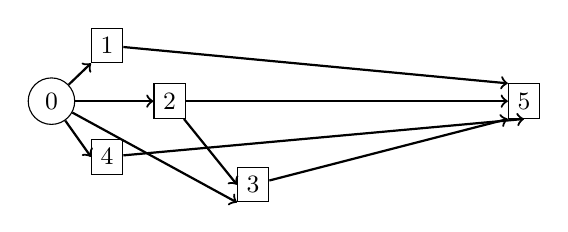
\begin{tikzpicture}
        [xscale=1.3]
        \node[draw,circle] (O) at (0,0) {\small $0$};
        \node[right of=O,draw,node distance=1.5cm] (D) {\small $2$}; 
        \node[above right of=O,draw] (U) {\small $1$}; 
        \node[below right of=D,draw,node distance =1.5cm] (T) {\small $3$}; 
        \node[below right of=O,draw] (Q) {\small $4$};
        \node[right of=D,draw,node distance=4.5cm] (C) {\small $5$};  

        \draw[->,thick] (O) -- (U.south west);
        \draw[->,thick] (O) -- (D.west);
        \draw[->,thick] (O) -- (T.south west);
        \draw[->,thick] (O) -- (Q.west) ;
        \draw[->,thick] (U) -- (C.north west) ;
        \draw[->,thick] (D) -- (C.west) ;
        \draw[->,thick] (D) -- (T.west) ;
        \draw[->,thick] (T) -- (C.south west) ;
        \draw[->,thick] (Q) -- (C.south) ;
      \end{tikzpicture}}
    \caption{Exemple d'instance pour le \RCPSP.} 
    \label{instance_ex_RCPSP}
  \end{figure}

  La figure~\ref{solution_ex_RCPSP_feas} présente un ordonnancement
  réalisable avec $C_{max}=15$. Cet ordonnancement n'est pas optimal
  puisque si l'activité $1$ est décalée à droite de manière à commencer
  au temps $t=8$, on peut décaler les trois autres activités vers la
  gauche et on obtient un ordonnancement ayant une date de fin
  inférieure à celle de l'ordonnancement précédent, i.e. $C_{max}=12$
  (cf. figure~\ref{solution_ex_RCPSP_opt}) dont on peut prouver
  l'optimalité.

  \begin{figure}[!htb]
    \centering
    \subcaptionbox{Une solution réalisable\label{solution_ex_RCPSP_feas}}[0.4\linewidth]{
      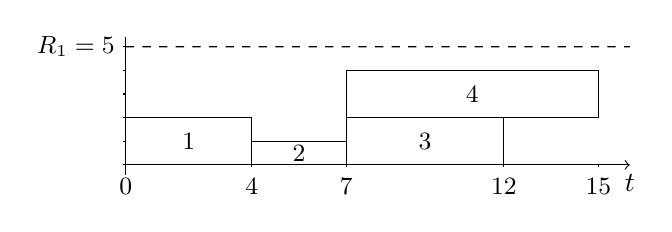
\begin{tikzpicture}
        [xscale=0.4,yscale=0.3]
        \node (O) at (0,0) {};
        \node (bmax) at (0,5) {};

        \draw[->] (O.center) -- (16,0) node[below] {$t$};
        \draw (O.south) -- (bmax.north);

        \draw[dashed] (bmax.center) node[left=0.5pt] {\small $R_1=5$} -- (16,5);
        \draw[fill=white] (0,0) rectangle (4,2) node[midway] {\small $1$};
        \draw[fill=white] (4,0) rectangle (7,1) node[midway] {\small $2$};
        \draw[fill=white] (7,0) rectangle (12,2) node[midway] {\small $3$};
        \draw[fill=white] (7,2) rectangle (15,4) node[midway] {\small $4$};

        \draw (0,0) -- (0,-0.1) node[below=0.5pt] {\small $0$};
        \draw (4,0) -- (4,-0.1) node[below=0.5pt] {\small $4$};
        \draw (7,0) -- (7,-0.1) node[below=0.5pt] {\small $7$};
        \draw (12,0) -- (12,-0.1) node[below=0.5pt] {\small $12$};
        \draw (15,0) -- (15,-0.1) node[below=0.5pt] {\small $15$};

        \foreach \i in {0,...,5}
        {\draw (0,\i) -- (-0.1,\i);}
      \end{tikzpicture}

      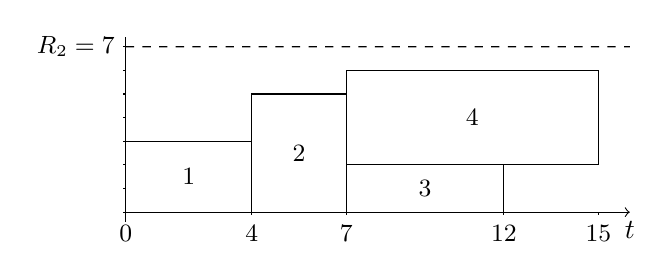
\begin{tikzpicture}
        [xscale=0.4,yscale=0.3]
        \node (O) at (0,0) {};
        \node (bmax) at (0,7) {};

        \draw[->] (O.center) -- (16,0) node[below] {$t$};
        \draw (O.south) -- (bmax.north);

        \draw[dashed] (bmax.center) node[left=0.5pt] {\small $R_2=7$} -- (16,7);
        \draw[fill=white] (0,0) rectangle (4,3) node[midway] {\small $1$};
        \draw[fill=white] (4,0) rectangle (7,5) node[midway] {\small $2$};
        \draw[fill=white] (7,0) rectangle (12,2) node[midway] {\small $3$};
        \draw[fill=white] (7,2) rectangle (15,6) node[midway] {\small $4$};

        \draw (0,0) -- (0,-0.1) node[below=0.5pt] {\small $0$};
        \draw (4,0) -- (4,-0.1) node[below=0.5pt] {\small $4$};
        \draw (7,0) -- (7,-0.1) node[below=0.5pt] {\small $7$};
        \draw (12,0) -- (12,-0.1) node[below=0.5pt] {\small $12$};
        \draw (15,0) -- (15,-0.1) node[below=0.5pt] {\small $15$};

        \foreach \i in {0,...,7}
        {\draw (0,\i) -- (-0.1,\i);}
      \end{tikzpicture}}
    \hfill
    \subcaptionbox{La solution optimale\label{solution_ex_RCPSP_opt}}[0.4\linewidth]{
      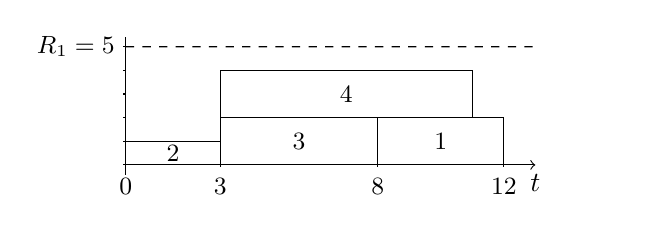
\begin{tikzpicture}
        [xscale=0.4,yscale=0.3]
        \node (O) at (0,0) {};
        \node (bmax) at (0,5) {};
        \node at (16,0) {};
        \draw[->] (O.center) -- (13,0) node[below] {$t$};
        \draw (O.south) -- (bmax.north);

        \draw[dashed] (bmax.center) node[left=0.5pt] {\small $R_1=5$} -- (13,5);
        \draw[fill=white] (0,0) rectangle (3,1) node[midway] {\small $2$};
        \draw[fill=white] (3,0) rectangle (8,2) node[midway] {\small $3$};
        \draw[fill=white] (3,2) rectangle (11,4) node[midway] {\small $4$};
        \draw[fill=white] (8,0) rectangle (12,2) node[midway] {\small $1$};

        \draw (0,0) -- (0,-0.1) node[below=0.5pt] {\small $0$};
        \draw (3,0) -- (3,-0.1) node[below=0.5pt] {\small $3$};
        \draw (8,0) -- (8,-0.1) node[below=0.5pt] {\small $8$};
        \draw (12,0) -- (12,-0.1) node[below =0.5pt] {\small $12$};

        \foreach \i in {0,...,5}
        {\draw (0,\i) -- (-0.1,\i);}
      \end{tikzpicture}

      \begin{tikzpicture}
        [xscale=0.4,yscale=0.3]
        \node (O) at (0,0) {};
        \node (bmax) at (0,7) {};
        \node at (16,0) {};

        \draw[->] (O.center) -- (13,0) node[below] {$t$};
        \draw (O.south) -- (bmax.north);

        \draw[dashed] (bmax.center) node[left=0.5pt] {\small $R_2=7$} -- (13,7);
        \draw[fill=white] (0,0) rectangle (3,5) node[midway] {\small $2$};
        \draw[fill=white] (3,3) rectangle (11,7) node[midway] {\small $4$};
        \draw[fill=white] (3,0) rectangle (8,2) node[midway] {\small $3$};
        \draw[fill=white] (8,0) rectangle (12,3) node[midway] {\small $1$};

        \draw (0,0) -- (0,-0.1) node[below=0.5pt] {\small $0$};
        \draw (3,0) -- (3,-0.1) node[below=0.5pt] {\small $3$};
        \draw (8,0) -- (8,-0.1) node[below=0.5pt] {\small $8$};    
        \draw (12,0) -- (12,-0.1) node[below=0.5pt] {\small $12$};

        \foreach \i in {0,...,7}
        {\draw (0,\i) -- (-0.1,\i);}
      \end{tikzpicture}}
    \caption{Exemple de solutions réalisables pour le \RCPSP.} 
    \label{solution_ex_RCPSP}
  \end{figure}
\end{ex}

Le \RCPSP~est un problème qui a été prouvé NP-complet au sens
fort~\cite{NP_RCPSP}. Ce problème a donc été très étudié dans la
littérature, notamment pour trouver des méthodes efficaces pour sa
résolution. Dans la section~\ref{sec:PLNE_ordo_res}, nous présentons des
modèles de programmation linéaire permettant de trouver la solution
optimale à ce problème. Ces modèles seront alors adaptés dans le cadre
d'un autre problème d'ordonnancement décrit dans le
paragraphe~\ref{sec:ordo_nrj}. 

\subsubsection{Le problème cumulatif}

Le problème d'ordonnancement cumulatif (CuSP) permet de caractériser
le fait que le projet implique une ressource (ou un sous-ensemble de
ressources) de nature cumulative. Le \CUSP~peut être vu comme un cas
particulier de la variante décisionnelle du RCPSP où l'on ne considère
qu'une ressource et où l'on remplace les contraintes de précédence par
les fenêtres de temps qu'elles induisent.

Formellement, le \CUSP~prend en entrée un ensemble $ \A=\{1,\dots,n\}$
d'activités non préemptives à ordonnancer. Pour s'exécuter, une
activité doit consommer une partie de la ressource $r_i$ et ce jusqu'à
l'arrêt de l'activité, i.e. après un temps $p_i$ correspondant à la
durée de l'activité $i$. Cette ressource est de type cumulatif,
discrète et renouvelable, disponible en quantité $R$.

De plus, chaque activité dispose d'une fenêtre de temps $[\ES,\LE]$
dans laquelle l'activité doit obligatoirement s'exécuter. Nous
rappelons que $\ES$ correspond à la date de début au plus tôt de $i$
et $\LE$ à sa date de fin au plus tard.

L'objectif du \CUSP~est donc de déterminer la date de début $st_i$ de
chaque activité $i \in \A$ telle que:
\begin{itemize}
\item la capacité de la ressource n'est excédée à aucun moment du
  projet, i.e.
  \begin{equation} \forall t \in \H,\sum_{\substack{i\in \A\\ t \in
        [st_i,st_i+p_i[}} r_{i} \le  R
\label{eq:CUSP_res}
\end{equation}
\item la fenêtre de temps de chaque activité est respectée, i.e. 
  \begin{equation} \forall i \in \A,\ \ES \le st_i < st_i+p_i \le \LE \end{equation}
\end{itemize}

Trouver une solution réalisable pour ce problème -- étant
une extension de la variante de décision du problème à une machine
($R=1$ et $r_i=1$) et du problème à $m$ machines ($R=m$ et $r_i=1$) -- 
est NP-complet au sens fort~\cite{NP_bible}. De ce fait, dans la
littérature, ce problème est souvent étudié sans fonction
objectif. Sauf précision du contraire, nous ferons de même dans la
suite du manuscrit. 

\begin{ex}
  \label{CUSP_ex}
  Considérons l'instance à quatre activités suivante:
  \begin{itemize}
  \item $R=4$
  \item cf. table~\ref{instance_CUSP_ex}\begin{table}[!htb]
      \centering
      \begin{tabular}{|P{1cm}|P{1cm}P{1cm}P{1cm}P{1cm}|}
        \hline
        i & p_i & \ES & \LE & r_i\\
        \hline
        1 & 2 & 1 & 5 & 2 \\
        2 & 1 & 3 & 5 & 2\\
        3 & 1 & 3 & 5 & 3\\
        4 & 4 & 1 & 10 & 1 \\
        \hline
      \end{tabular}
      \caption{Exemple d'une instance du \CUSP.}
      \label{instance_CUSP_ex}
    \end{table}
  \end{itemize}
  La figure~\ref{solution_CUSP_ex} présente plusieurs solutions
  réalisables pour cette instance. 
  \begin{figure}
    \begin{minipage}{0.45\linewidth}
      \begin{tikzpicture}
        [xscale=0.6,yscale=0.7]
        \node (O) at (0,0) {};
        \node (bmax) at (0,3) {};
        \node at (9,0) {};

        \draw[->] (O.center) -- (9,0) node[below] {$t$};
        \draw (O.south) -- (bmax.north);

        \draw[dashed] (bmax.center) node[left=0.5pt] {\small $R=3$} -- (9,3);
        \draw[fill=white] (1,0) rectangle (3,2) node[midway] {\small $1$};
        \draw[fill=white] (3,0) rectangle (4,3) node[midway] {\small $3$};
        \draw[fill=white] (4,2) rectangle (8,3) node[midway] {\small $4$};
        \draw[fill=white] (4,0) rectangle (5,2) node[midway] {\small $2$};

        \draw (1,0) -- (1,-0.1) node[below=0.5pt] {\small $1$};
        \draw (3,0) -- (3,-0.1) node[below=0.5pt] {\small $3$};
        \draw (5,0) -- (5,-0.1) node[below=0.5pt] {\small $5$};    
        \draw (4,0) -- (4,-0.1) node[below=0.5pt] {\small $4$}; 
        \draw (8,0) -- (8,-0.1) node[below=0.5pt] {\small $8$};

        \node at (10,0) {};
        \foreach \i in {0,...,3}
        {\draw (0,\i) -- (-0.1,\i);}
      \end{tikzpicture}
    \end{minipage}
    \hfill
    \begin{minipage}{0.45\linewidth}
      \begin{tikzpicture}
        [xscale=0.6,yscale=0.7]
        \node (O) at (0,0) {};
        \node (bmax) at (0,3) {};
        \node at (10,0) {};

        \draw[->] (O.center) -- (10,0) node[below] {$t$};
        \draw (O.south) -- (bmax.north);

        \draw[dashed] (bmax.center) node[left=0.5pt] {\small $R=3$} -- (10,3);
        \draw[fill=white] (1,0) rectangle (3,2) node[midway] {\small $1$};
        \draw[fill=white] (4,0) rectangle (5,3) node[midway] {\small $3$};
        \draw[fill=white] (5,2) rectangle (9,3) node[midway] {\small $4$};
        \draw[fill=white] (3,0) rectangle (4,2) node[midway] {\small $2$};

        \draw (1,0) -- (1,-0.1) node[below=0.5pt] {\small $1$};
        \draw (3,0) -- (3,-0.1) node[below=0.5pt] {\small $3$};
        \draw (5,0) -- (5,-0.1) node[below=0.5pt] {\small $5$};    
        \draw (4,0) -- (4,-0.1) node[below=0.5pt] {\small $4$}; 
        \draw (8,0) -- (8,-0.1) node[below=0.5pt] {\small $8$};

        \foreach \i in {0,...,3}
        {\draw (0,\i) -- (-0.1,\i);}
      \end{tikzpicture}
    \end{minipage}
    \caption{Exemple de solutions réalisables pour le \CUSP.}
    \label{solution_CUSP_ex}
  \end{figure}
\end{ex}

Dans la section~\ref{sec:cumu}, nous présenterons des
méthodes de résolution pour ce problème utilisant la programmation par
contraintes. 

\subsubsection{Limites des problèmes cumulatifs en termes de modélisation}
\label{sec:limit_CUSP}
Une des principales limitations du \RCPSP~et donc du \CUSP~(qui en est
un cas particulier) en termes de modélisation est que, dans ces
problèmes, chaque activité consomme une quantité de ressource fixe,
connue à l'avance, durant toute sa durée d'exécution. De plus, cette
durée est aussi supposée fixe. Cependant, pour de nombreux problèmes
pratiques, ces suppositions reviennent à sur-contraindre le
problème. En effet, considérons l'exemple suivant, décrit
dans~\cite{FT}.  Dans cet exemple, une activité représentant la
peinture d'un bateau est considérée. Pour cette activité, la durée est
remplacée par une quantité de travail, ou énergie, représentant le
travail de $3$ personnes sur une journée. Cette activité peut, au
choix, être exécutée en $3$ jours par $1$ personne, ou en $2$ jours
par $2$ personnes le premier jour et $1$ personne le second, ou encore
par $3$ personnes en seulement un jour. Si l'on avait supposé une
consommation et une durée fixe, l'espace des solutions aurait été
réduit.

L'exemple décrit ci-dessus peut facilement être généralisé à de
nombreux cas pratiques. Un autre exemple venant d'un problème
industriel est présenté dans~\cite{HaitArtiguesLopez}. Dans cet
article, une application dans une fonderie où du métal est fondu dans
des fournaises à induction est détaillé. La puissance de chaque
fournaise utilisée pour faire fondre le métal peut être réglée, à tout
moment, afin d'éviter un dépassement d'un certain niveau d'énergie
(généralement dû à une limite suggérée par le fournisseur
d'énergie). De ce fait, si chaque opération de fonte est vue comme une
activité, nous avons besoin de pouvoir moduler la quantité d'énergie
donnée à cette activité à chaque instant et la durée de l'activité
dépend de cette quantité d'énergie.

Pour représenter ces variations dans le profil de consommation des
activités, nous avons choisi de modéliser la ressource comme une
ressource continue. En effet, de nombreux exemples de ressource
continue existent. C'est le cas de l'électricité, des sources
d'énergie hydrauliques, du carburant ou encore de la mémoire d'un
ordinateur. D'autres ressources telles que des employés ou des
machines, qui sont normalement modélisées à l'aide de ressources
discrètes, peuvent être modélisées par des ressources continues si
l'on suppose qu'un employé ou une machine peut exécuter plusieurs
activités en parallèle~\cite{W80,NK}.

De plus, les problèmes à ressources continues peuvent aussi servir de
relaxation pour les problèmes avec des ressources discrètes. En effet,
le caractère discret du problème peut parfois amener à considérer de
nombreuses possibilités d'affectations de la ressource. Ce grand nombre
d'affectation peut grandement complexifier le problème. Donc,
considérer des ressources continues peut permettre l'agrégation des
raisonnements dédiés à ces problèmes. 

La modélisation complète du problème considéré dans cette thèse est
décrit dans la section suivante. Cette modélisation sera ensuite
comparée aux extensions du \CUSP~et du \RCPSP, déjà existantes dans la
littérature. 

